\documentclass{article}


% if you need to pass options to natbib, use, e.g.:
%     \PassOptionsToPackage{numbers, compress}{natbib}
% before loading neurips_2021

% ready for submission
\usepackage[preprint]{neurips_2021}
\bibliographystyle{abbrvnat}

\usepackage[utf8]{inputenc} % allow utf-8 input
\usepackage[T1]{fontenc}    % use 8-bit T1 fonts
\usepackage[colorlinks=true]{hyperref}       % hyperlinks
\usepackage{url}            % simple URL typesetting
\usepackage{booktabs}       % professional-quality tables
\usepackage{amsfonts}       % blackboard math symbols
\usepackage{nicefrac}       % compact symbols for 1/2, etc.
\usepackage{microtype}      % microtypography
\usepackage{xcolor}         % colors
\usepackage{siunitx}
\usepackage{graphicx}

\newcommand{\todo}[1]{{\color{red} #1}}

\title{Spotify feat. Logistic Regression - \\ Popularity, Nothing Else Matters}

% The \author macro works with any number of authors. There are two commands
% used to separate the names and addresses of multiple authors: \And and \AND.
%
% Using \And between authors leaves it to LaTeX to determine where to break the
% lines. Using \AND forces a line break at that point. So, if LaTeX puts 3 of 4
% authors names on the first line, and the last on the second line, try using
% \AND instead of \And before the third author name.

\author{%
  Sebastian Hoffmann\thanks{correspondence to \texttt{sebastian.hoffmann@student.uni-tuebingen.de}}\\
  Matrikelnummer 5954377
  \And
  Yannick Streicher\thanks{correspondence to \texttt{yannick.streicher@student.uni-tuebingen.de}}\\
  Matrikelnummer 5331817
}

\begin{document}

\maketitle

\begin{abstract}
  What is the musical taste of the world? With the recent rise and global pervasiveness of music streaming services, such as Spotify, Deezer, or Apple Music, answering this question has become tractable. For this, we plan to analyze a \href{https://www.kaggle.com/rodolfofigueroa/spotify-12m-songs}{subset of 1.2 million songs} scraped from Spotify. However, this dataset lacks crucial information about popularity. Thus, an important step of our work is to augment the dataset further by querying the official Spotify REST API for a randomly sampled subset of the data. Besides a birds-eye overview of the musical landscape, e.g. distribution of genres, we want to identify common musical properties shared by popular songs, and likewise, very unpopular songs, using logistic regression. Such properties can be, for instance, tempo, mode, or key.
\end{abstract}

\section{Introduction}
The large amount of digital music today can be daunting. To successfully navigate this space, we urgently need better knowledge of the key characteristics of this opaque, highdimensional space. With our work, we want to present two important findings that contribute to this goal in a twofold manner: \textit{First} we create a clear overview of the musical landscape. That is, by applying t-SNE (\todo{cite?}) we show a twodimensional embedding of the high dimensional space of audio tracks. We find clusters that can be labeled as musical \textit{genres}. \textit{Second}, we zoom in and, using logistic regression, distill audio features that are of particular interest when considering the popularity of an audio track.

To pursue our overall goal of predicting the popularity of a song given its Spotify features, we have to find good labels that discriminate popular and unpopular songs. However, the Kaggle dataset\footnote{include link} only contains musical song features. Spotify\footnote{link company} includes some metrics that summarize a measure of popularity, derived by preferences of Spotify's users. In the end, two metrics are important for our project, \textit{(i): Popularity:} An integer between 0 and 100 describing how popular a track is. According to Spotify's API description, this metric is determined algorithmically based on the total number of plays a track has, as well as, how recent those plays are. Artist popularity is derived from the popularity of its individual tracks. The second feature is \textit{(ii): Followers} which is the number of accounts that subscribed to this artists Spotify feed. The number can be interpreted as peoples interest in following the new releases of a particular artist.

\section{Filtering and Preprocessing}

The starting point for the project was the 1.2m song dataset on Kaggle. For all of those songs, we queried the Spotify API for additional artist information. In total, we queried around \num[]{85 000} artists, each having a popularity score and a number of followers. Additionally, each artist is described by a set of genres.

With the advent of online self-publishing, it became very easy and accessible to distribute home-produced music to a worldwide audience. In fact, there exist specialized companies, such as TuneCore or DistroKid for instance, that automatically distribute submitted songs to multiple platforms at the same time, including Spotify and Apple Music. Indeed we find that a quarter of artists on Spotify have less than $45$ followers and half of all artist have less than $393$. For comparison, \emph{Merikan}, a relatively unknown \emph{Drum and Bass} producer, which is not a major genre, has $4581$ follower at the time of writing. Given that self-published songs do not undergo the feedback and quality control process a regular music label would provide to an artist, we are worried that these tracks can potentially introduce a lot of noise to our data. Consequently, we filter our dataset to only include songs of artists that are to some extent known and established and can be considered professional or semi-professional musicians.

There are two metrics that could potentially be considered as a filter criterion: The popularity of an artist and the number of followers. We find that the number of followers is roughly exponentially distributed. After transforming it logarithmically, there is a clear linear relationship between the number of (log) followers and popularity visible (Pearson correlation coefficient: $0.88$, see Figure~\ref{fig:filtering}~left). This indicates that a more robust measure can be derived by combining both metrics into one.

To this end, we transform both followers and popularity using PCA. The first principal component can be seen as a robust measure of artist popularity, whereas the second component indicates the deviation from the linear relationship. Upon further inspection, we find artists such as \emph{\todo{find the minecraft guy}} that while having a significant amount of followers, do not have any successful songs. To further reduce noise, we filter these outliers as well by thresholding the second principal component. This affects $1366$ artists ($1.6\%$). We then threshold the first component to filter $50\%$ of all artists. Finally, we filter all artists that do not have a genre associated with them (affects $52.26\%$\footnote{Notice that there is a big overlap with unknown artists, presumably since scarce data makes it difficult for Spotify to establish a genre.}).

In total, if all three steps are applied, $62.8\%$ of all artists are removed from the dataset and $31694$ artists in total are retained. This reduces the number of songs left in the dataset to $755472$, or $62.75\%$ of the original size.

\begin{figure}
  \centering
  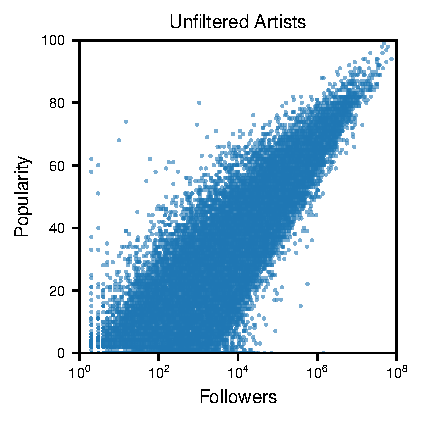
\includegraphics[width=0.42\textwidth]{../figures/artists_unfiltered.pdf}
  \qquad
  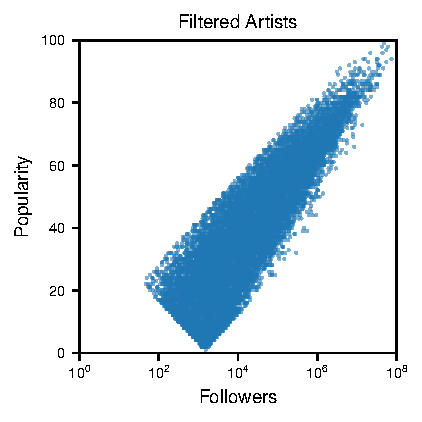
\includegraphics[width=0.42\textwidth]{../figures/artists_filtered.pdf}
  \caption{\textit{Left}: Artist popularity against log-followers before applying our filtering rules. \textit{Right}: We use the result of PCA to exclude artists that are outliers with respect to the first and second principal component.}
  \label{fig:filtering}
\end{figure}

\section{Dimensionality Reduction - Clustering Song Genres}

\begin{figure}
  \centering
  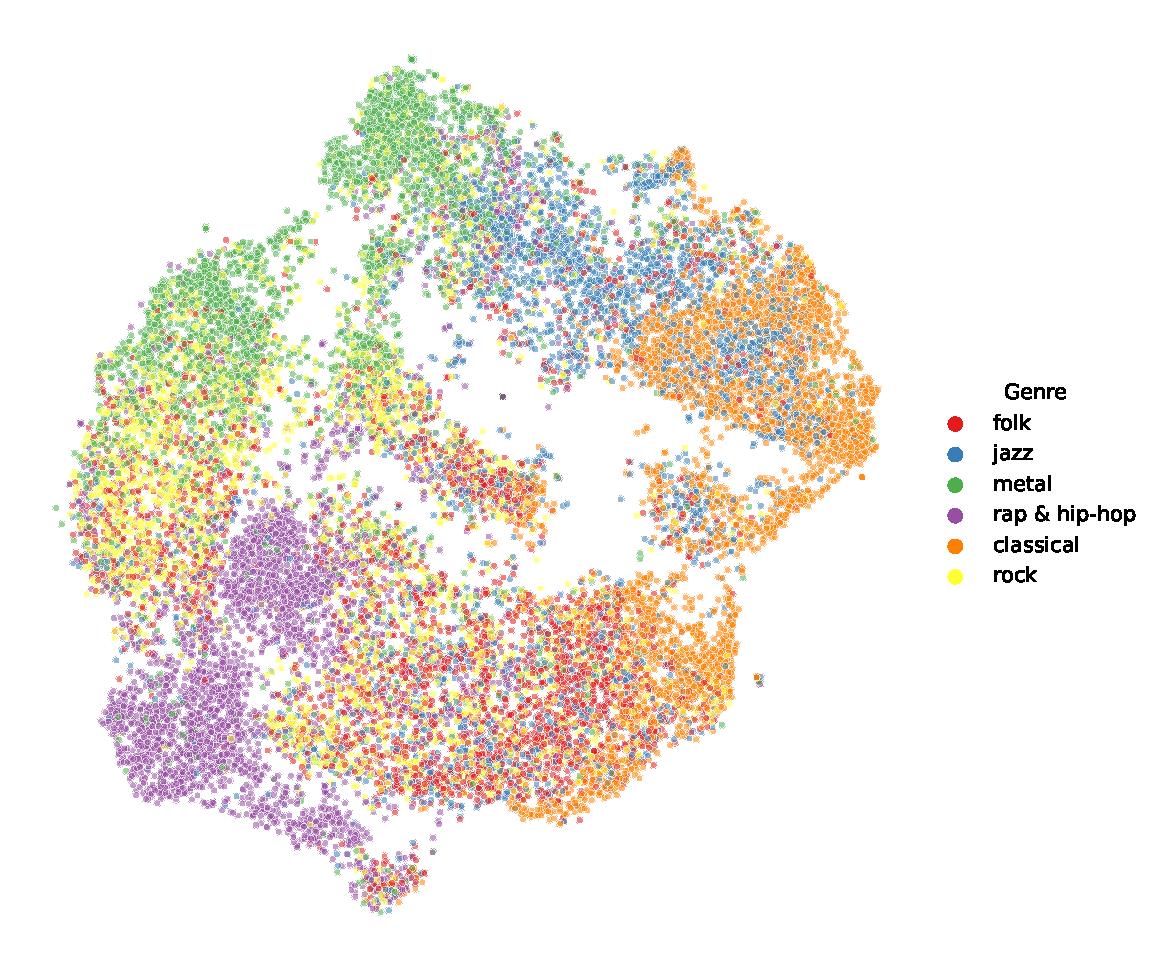
\includegraphics[width=0.8\textwidth]{../figures/tsne_genres.pdf}
  \caption{tsne}
  \label{fig:tsne_genres}
\end{figure}

\begin{itemize}
  \item Some homogeneous clusters arise, such as rap, classical music and metal. 
  \item Cluster neighborhoods are interesting. For instance, jazz is neighbor of classical.
  \item Also, a lot of songs are really mixed.
\end{itemize}

\section{Statistical Analysis - Logistic Regression}
For this project, our variable of interest is beeing \textit{popular} vs. \textit{unpopular} for individual tracks.
For the prediction we consider the \textit{audio features} for each of the tracks. 
Those features are purely technical and, therefore, we inductively assume that the probability whether a song is popular is only dependent on its audio features. 

To create the labels, we apply a threshold to the popularity measure. 
We perform two different experiments. 
One tight threshold, labeling only the top \SI{10}{\percent} songs as popular, and one more general one where we use the median to divide the track into two groups.
To train the classifier we divide the dataset into \SI{80}{\percent} training and \SI{20}{\percent} test data.
As the tight threshold dataset contains a lot more unpopular songs than popular songs, the corresponding logistic regression model easily gets stuck in predicting \textit{unpopular} for all training examples. 
To address this issue, we follow the state of the art and use a \textit{weighted loss} function to penalize this behavior~\cite{haixiangLearningClassimbalancedData2017a}.

For both logistic regression models we apply l2-regularization and select the best hyperparameters via grid search, using 5-fold cross validation. Then, the final models are evaluated on individual test sets, respecting their popularity threshold.
At first it seems that the tight model performs better then the wide model, getting an AUC score of \num{0.73} vs. \num{0.68} for the wide model.
%
However, if we look closer on how the predictions are distributed (see the calibration plots in Fig.~\ref{fig:logis_eval}), we clearly see that the tight model highly overestimates the probability of beeing popular.

Since we aim to predict popularity in general, and not to be a real chart striker, we decided to accept the more general model.
To find out how each features influence the prediction we look into the learned coefficients of our regression model, c.f.~Fig.\ref{fig:logis_eval}.
Weights in logistic regression have a linear relationship with the \textit{odds} of an outcome of the target variable.
Our analysis shows, that especially \textit{loudness} and \textit{danceability} correspond to a higher odds of beeing popular.
These findings align with phenomena such as the \textit{loudness war}\footnote{reference} of recorded music which emerged in the last years.
Finding that \textit{danceability} correlates with higher odds of beeing popular could be pontentially be an indication that gives hints to the answer of our overall thesis - the humankind seems to like music that can be danced on.
On the flip side we also have negative correlations. 
Acousticness and instrumentalness negatively predict the odds, as well as valence and energy (which are correlated by 0.42 and have a similar interpretation).


\begin{figure}
  %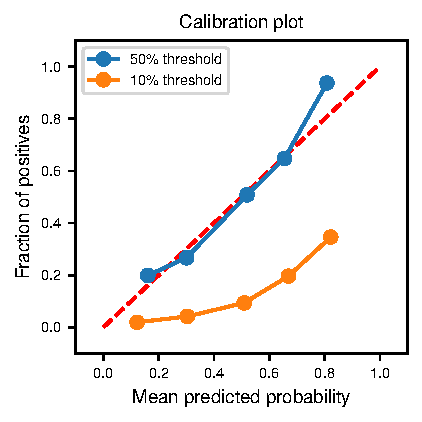
\includegraphics[width=0.42\textwidth]{../figures/calibration_combined.pdf}
  %\qquad
  %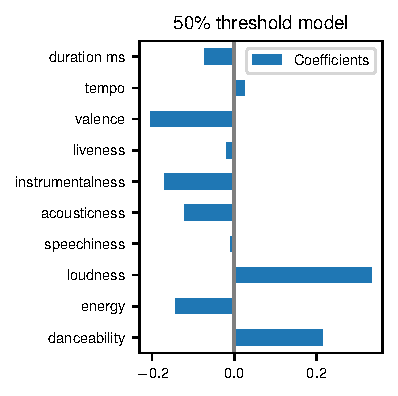
\includegraphics[width=0.42\textwidth]{../figures/logistic_coefs_50_threshold_model.pdf}
  \caption{\textit{Left}: Calibration plot following the methodology of \cite{niculescu-mizilPredictingGoodProbabilities2005}. The prediction space is discretized into 5 bins. Using the test set, for each bin, we plot the fraction of true popular songs against the mean predicted probability for those songs. \textit{Right}: The coefficients of the selected model for each audio feature. For the interpretation of individual features consider the API documentation of Spotify.}
  \label{fig:logis_eval}
\end{figure}

% \begin{figure}
%   \centering
%   \includegraphics[width=0.42\textwidth]{../figures/roc_logistic.pdf}
%   \caption{Parameters}
%   \label{fig:params}
% \end{figure}
  

\section{Discussion}
Our work is limited because\dots
In regards to ... we cannot estimate confidence because ...

\begin{itemize}
  \item Using multiclass logistic regression suffers from the issue that the top classes are highly imbalanced in contrast to the unpopular classes. Using weight based approaches for the loss function leads bad performances for the classes of the highly rare events (exp 007). 
  \item it is somehow adversarial that energy and valence negativly predict the odds, while danceability positively predict the odds, while for instance valence and danceability are correlated by 0.59.
\end{itemize}

\begin{itemize}
  \item For the more tight model, we have way less training examples for the popular group, then with the more general model. This could be a potential reason for the shifted distribution.
  \item Song features lack important factors that correlate with song popularity, e.g., is the name of the artist relevant in pop culture. For the analysis we assumed that song popularity is discriminated by features that are only related on the "physical properties" of the song. However, for predicting popularity we might have to respect some "marketing aspects" as well. 
\end{itemize}


% not working, why?
% \bibliography{bibliography}
%\printbibliography
\bibliography{bibliography}

\end{document}
